\documentclass[11pt, oneside]{article}
\usepackage[margin=1in,letterpaper]{geometry}
\usepackage{times}
\usepackage{graphicx}
\usepackage{amssymb,amsmath}
\usepackage{array}
\usepackage{longtable}
\usepackage{color}
\usepackage[T1]{fontenc}
\usepackage{sectsty}
\usepackage{tikz}
\usepackage{pgfplots}
\pgfplotsset{compat=1.17}
\sectionfont{\fontsize{12}{12}\selectfont}
\subsectionfont{\fontsize{11}{11}\selectfont}
\subsubsectionfont{\normalsize\itshape\mdseries}

\renewcommand\labelitemi{{\boldmath$\cdot$}}

%%%%%%%%%%%%%%%%%%%%%%%%%%%%%%%%%%%%%
% Notation: vectors are bold (handwritten: underlined); unit vectors are \hat{\mathbf{x}}, etc.
% Following the master table (D2, D12), phasors carry a tilde: E(x,y,z,t) = Re[E~(x,y,z) e^{jwt}].
% Per the master table: phase velocity u_p (D15), wavenumber lowercase k (D14), Poynting vector in script S (D10);
% the handwriting uses v_p, capital K, and a plain S. The handwritten loop length l is written \ell.
% The handwriting writes the string waves with e^{j(kz - wt)}; converted to the course convention e^{j(wt - kz)}.
% Symbols flagged as pending dual usages in the master table: T (D19), m (D20), f (D21), A (D22),
% superscripts/subscripts I, R, T vs i, r, t (D23), delta (D24), S and P for surface/loop (D25, D26),
% E_0^i (D27), media subscripts 1, 2 (D28), tau (D18).
%%%%%%%%%%%%%%%%%%%%%%%%%%%%%%%%%%%%%

\title{Ge158 Lecture 4: EM Wave Transmission and Reflection at Planar Interfaces, Part 1: Normal Incidence}
\author{Brent Minchew}
\date{}

\begin{document}
\maketitle

\noindent\textbf{Topics covered}
\begin{itemize}
	\item Transverse waves on strings as an analog for EM waves
	\item Boundary conditions for transverse waves
	\item EM waves with normal incidence to a plane
	\item EM boundary conditions
	\item Fresnel equations for normal incidence
\end{itemize}

%%%%%%%%%%%%%%%%%%%%%%%%%%%%%%%%%%%%%
% NOTE (notation, instructor decisions 2026-09-29, master table D19--D24, D26, D27): handwritten string displacement f,
% amplitudes A_I, A_R, A_T, phases delta_I, delta_R, delta_T, tension T, mass per length m, loop P, amplitudes E_0^i, E_0^r, E_0^t,
% reflectivity R and transmissivity T are written xi, xi_0^i..., phi^i..., F_tension, m_ell, dA, E^i..., Gamma, and blackboard T.
% Integration surfaces (handwritten S): closed surface dV (boundary of volume V) for Gauss's laws; open surface A
% bounded by the loop dA (handwritten P) for Faraday's and Ampere's laws (D25, D26).
\section{Transverse waves on a string}

Let's start with some intuition building by considering the canonical example of waves on strings.

\subsection{Longitudinal and transverse waves}

There are two types of waves:
\begin{itemize}
	\item \emph{longitudinal waves} (e.g., sound waves, stretching of a Slinky, etc.);
	\item \fbox{\emph{transverse waves} (e.g., waves generated by shaking or plucking strings).}
	% NOTE: handwritten reads "EM waves are always transverse"; qualified to plane waves, as in Lecture 2
	% (Ulaby & Long 2014, p. 39, TEM waves).
	\begin{itemize}
		\item[$\hookrightarrow$] EM (plane) waves are \emph{always} transverse.
	\end{itemize}
\end{itemize}

Recall the wave equation for a wave traveling in the $z$ direction,
\begin{equation}
	\frac{\partial^2 \xi}{\partial z^2} = \frac{1}{u_p^2}\frac{\partial^2 \xi}{\partial t^2},
\end{equation}
where $\xi(z,t)$ is the (transverse) displacement of the string. For a string, you may recall from physics classes that
\begin{equation}
	u_p = \sqrt{\frac{F_\mathrm{tension}}{m_\ell}},
\end{equation}
where $F_\mathrm{tension}$ is the tension of the string and $m_\ell$ is its mass per unit length. (For EM waves, we showed before that $u_p = c/n'$, where $n' = \mathrm{Re}(\sqrt{\varepsilon})$; Lecture 2.)

\subsection{Two strings joined at $z = 0$}

Let us consider two strings attached at $z = 0$: string 1 extends to $z\to-\infty$ and string 2 to $z\to+\infty$.
\begin{itemize}
	\item $F_{\mathrm{tension},1} = F_{\mathrm{tension},2}$;
	\item $m_{\ell 1} \ne m_{\ell 2} \Rightarrow u_{p1} \ne u_{p2}$ (just as we'd expect for EM waves when $\varepsilon_1 \ne \varepsilon_2$).
\end{itemize}

% NOTE: handwritten writes the waves as A e^{j(kz - wt)} (physics convention e^{-jwt}) with capital K;
% converted to the course convention e^{jwt} (master table, Conventions), i.e., A e^{j(wt - kz)}, and lowercase k (D14).
% Both forms describe the same waves, and the boundary conditions give the same A_R and A_T.
An incident wave traveling in the $+z$ direction in string 1,
\begin{equation}
	\xi^i = \xi_0^i\,e^{j(\omega t - k_1 z)} \qquad (\text{string 1},\ z<0),
\end{equation}
gives a reflected wave (traveling in the $-z$ direction in string 1)
\begin{equation}
	\xi^r = \xi_0^r\,e^{j(\omega t + k_1 z)} \qquad (\text{string 1},\ z<0)
\end{equation}
and a transmitted wave (traveling in the $+z$ direction in string 2)
\begin{equation}
	\xi^t = \xi_0^t\,e^{j(\omega t - k_2 z)} \qquad (\text{string 2},\ z>0).
\end{equation}

\begin{itemize}
	\item The frequency $\omega$ must be the same everywhere and is set by the source (e.g., the person shaking the string, the RS instrument, etc.).
	\item Recalling the dispersion relation, $\omega = k u_p$: if $m_{\ell 1} \ne m_{\ell 2}$, then $u_{p1} \ne u_{p2}$ and $k_1 \ne k_2$.
	\item[] $\Rightarrow$ the wavelength must differ if $m_{\ell 1} \ne m_{\ell 2}$.
\end{itemize}

Now let us define the net displacement in each string:
\begin{equation}
	\label{e:string}
	\xi(z,t) =
	\begin{cases}
		\xi_0^i\,e^{j(\omega t - k_1 z)} + \xi_0^r\,e^{j(\omega t + k_1 z)} & \text{for } z<0,\\[4pt]
		\xi_0^t\,e^{j(\omega t - k_2 z)} & \text{for } z>0.
	\end{cases}
\end{equation}

\subsection{Boundary conditions and reflection and transmission}

Define the boundary conditions (BCs) at $z = 0$:
\begin{enumerate}
	\item $\xi(z=0^-,t) = \xi(z=0^+,t)$; otherwise, the strings would be disconnected.
	\item $\left.\dfrac{\partial \xi}{\partial z}\right|_{0^-} = \left.\dfrac{\partial \xi}{\partial z}\right|_{0^+}$; otherwise, there would need to be a net force acting at $z = 0$.
\end{enumerate}
Applying the BCs to Eq.~\eqref{e:string}, we have
\begin{equation}
	\xi_0^i + \xi_0^r = \xi_0^t
	\qquad \text{and} \qquad
	k_1(\xi_0^i - \xi_0^r) = k_2 \xi_0^t.
\end{equation}
In RS, we often know $\xi_0^i$, so we rearrange to get
\begin{align}
	\xi_0^r &= \left(\frac{k_1 - k_2}{k_1 + k_2}\right)\xi_0^i = \left(\frac{u_{p2} - u_{p1}}{u_{p2} + u_{p1}}\right)\xi_0^i, \\
	\xi_0^t &= \left(\frac{2k_1}{k_1 + k_2}\right)\xi_0^i = \left(\frac{2u_{p2}}{u_{p2} + u_{p1}}\right)\xi_0^i.
\end{align}
As we went over with EM waves, $\xi_0^i$, $\xi_0^r$, and $\xi_0^t$ can be complex-valued, and we can write them in terms of magnitude and phase ($\phi^i$, $\phi^r$, $\phi^t$) as
\begin{equation}
	\label{e:string_phase}
	|\xi_0^r|e^{j\phi^r} = \left(\frac{u_{p2} - u_{p1}}{u_{p2} + u_{p1}}\right)|\xi_0^i|e^{j\phi^i},
	\qquad
	|\xi_0^t|e^{j\phi^t} = \left(\frac{2u_{p2}}{u_{p2} + u_{p1}}\right)|\xi_0^i|e^{j\phi^i}.
\end{equation}

Important take-aways from Eqs.~\eqref{e:string_phase}:
\begin{itemize}
	\item Continuity requires $\phi^t = \phi^i$.
	\item But Eqs.~\eqref{e:string_phase} require
	\begin{equation}
		\phi^r =
		\begin{cases}
			\phi^i - \pi & \text{for } u_{p1} > u_{p2} \quad \text{(reflected wave upside down)},\\
			\phi^i & \text{for } u_{p2} > u_{p1} \quad \text{(reflected wave right side up)}.
		\end{cases}
	\end{equation}
	% NOTE: handwritten reads "in the EM case, sigma_2 >> sigma_1"; corrected because that is not sufficient for total reflection:
	% with air above (sigma_1 = 0) any sigma_2 > 0 satisfies it, yet dry soil (eps' = 4, sigma = 1e-4 S/m, 1 GHz) gives rho = -0.33.
	% Near-total reflection needs |eps_2| >> |eps_1| (Eq. e:fresnel).
	\item If $m_{\ell 2} \gg m_{\ell 1}$ (similarly, if string 2 is fixed in place or, in the EM case, $|\varepsilon_2| \gg |\varepsilon_1|$, e.g., $\sigma_2/(\omega\varepsilon_0) \gg \varepsilon_1'$), then
	\begin{equation}
		u_{p2} \ll u_{p1} \quad\Rightarrow\quad |\xi_0^r| \approx |\xi_0^i| \quad \text{and} \quad |\xi_0^t| \approx 0.
	\end{equation}
\end{itemize}

%%%%%%%%%%%%%%%%%%%%%%%%%%%%%%%%%%%%%
\section{EM boundary conditions}

Having developed our intuition using the string analogy, let's move to EM waves. First, let's derive the BCs.

\subsection{Maxwell's equations in integral form}

% NOTE: handwritten margin note labels the closed-surface integral in Gauss's law as a "line integral over closed loop";
% corrected: the circle on the integral sign denotes integration over a closed surface S here and over a closed loop P
% in Faraday's and Ampere's laws below.
% NOTE: the handwritten underlined vector a (normal) is written as the unit normal \hat{a}. Brief clarifications not in
% the handwriting (unflagged elsewhere): the definition of f(z,t) as the transverse displacement, the "(Lecture 2)" pointers,
% and the explanatory sentences in the captions of Figs. 1 and 2.
Gauss's laws are integrals over any closed surface $\partial\mathcal{V}$ (the boundary of a volume $\mathcal{V}$) with normal $\hat{\mathbf{a}}$ (positive pointing from medium 2 to medium 1), where the circle on the integral sign denotes a \emph{closed} surface:
\begin{align}
	\oint_{\partial\mathcal{V}} \varepsilon'\varepsilon_0\,\mathbf{E}\cdot d\mathbf{a} &= 0 \qquad \text{(Gauss's law)}, \\
	\oint_{\partial\mathcal{V}} \mu\,\mathbf{H}\cdot d\mathbf{a} &= 0 \qquad \text{(Gauss's law for magnetism)}.
\end{align}
Faraday's and Amp\`ere's laws hold for any open surface $\mathcal{A}$ bounded by a closed loop $\partial\mathcal{A}$:
% NOTE: handwritten writes dH/dt and dE/dt inside the surface integrals; written as partial derivatives.
\begin{align}
	\oint_{\partial\mathcal{A}} \mathbf{E}\cdot d\boldsymbol{\ell} &= -\mu\int_{\mathcal{A}} \frac{\partial\mathbf{H}}{\partial t}\cdot d\mathbf{a} \qquad \text{(Faraday's law)}, \\
	\oint_{\partial\mathcal{A}} \mathbf{H}\cdot d\boldsymbol{\ell} &= I_f + \varepsilon'\varepsilon_0\int_{\mathcal{A}} \frac{\partial\mathbf{E}}{\partial t}\cdot d\mathbf{a} \qquad \text{(Amp\`ere's law)},
\end{align}
where $I_f$ is the free current passing through the loop, taken to be $I_f = 0$ hereafter.

\subsection{Gauss's law}

Let's consider a very thin pillbox centered on the interface between two media and extending slightly into each (Figure~\ref{f:pillbox}).

\begin{figure}[h]
	\centering
	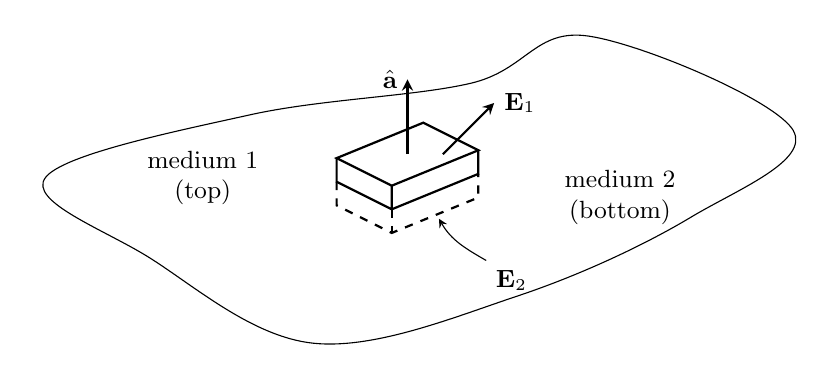
\begin{tikzpicture}[>=stealth, font=\small]
		% interface (irregular sheet)
		\draw[thin] plot[smooth cycle, tension=0.6] coordinates {(-4.6,0.1) (-2.0,0.9) (0.8,1.3) (2.3,1.9) (4.9,0.7) (3.6,-0.4) (1.4,-1.4) (-1.2,-2.0) (-3.3,-0.9)};
		\node[align=center] at (-2.6,0.1) {medium 1\\(top)};
		\node[align=center] at (2.7,-0.15) {medium 2\\(bottom)};
		% pillbox: upper half (solid, medium 1)
		\coordinate (T1) at (-0.9,0.35);
		\coordinate (T2) at (0.2,0.80);
		\coordinate (T3) at (0.9,0.45);
		\coordinate (T4) at (-0.2,0.00);
		\coordinate (M1) at (-0.9,0.05);
		\coordinate (M3) at (0.9,0.15);
		\coordinate (M4) at (-0.2,-0.30);
		\coordinate (B1) at (-0.9,-0.25);
		\coordinate (B3) at (0.9,-0.15);
		\coordinate (B4) at (-0.2,-0.60);
		\draw[thick] (T1) -- (T2) -- (T3) -- (T4) -- cycle;
		\draw[thick] (T1) -- (M1) -- (M4) -- (T4);
		\draw[thick] (M4) -- (M3) -- (T3);
		% pillbox: lower half (dashed, below the interface in medium 2)
		\draw[thick, dashed] (M1) -- (B1) -- (B4) -- (B3) -- (M3);
		\draw[thick, dashed] (M4) -- (B4);
		% normal and fields
		\coordinate (C) at (0.0,0.40);
		\draw[->, thick] (C) -- (0.0,1.35) node[left] {$\hat{\mathbf{a}}$};
		\draw[->, thick] (0.45,0.40) -- (1.10,1.05) node[right] {$\mathbf{E}_1$};
		\draw[->, thin] (1.0,-0.95) node[below right] {$\mathbf{E}_2$} to[out=150,in=-60] (0.40,-0.42);
	\end{tikzpicture}
	\caption{A thin pillbox straddling the interface between medium 1 (top) and medium 2 (bottom), with normal $\hat{\mathbf{a}}$. The part of the box in medium 2 is dashed.}
	\label{f:pillbox}
\end{figure}

From Gauss's law, we have
\begin{equation}
	\varepsilon_1'\mathbf{E}_1\cdot\hat{\mathbf{a}} = \varepsilon_2'\mathbf{E}_2\cdot\hat{\mathbf{a}}
\end{equation}
(note that the edges of our pillbox contribute nothing as the thickness of the box $\rightarrow 0$). Since $\hat{\mathbf{a}}$ is the normal,
% NOTE: handwritten defines the generic "E_i^perp"; written for media 1 and 2 explicitly because i denotes "incident"
% later in this lecture (and "ice" in Lecture 1).
\begin{equation}
	\boxed{\varepsilon_1'E_1^\perp = \varepsilon_2'E_2^\perp}
\end{equation}
where $E_1^\perp$ and $E_2^\perp$ denote the components of the $\mathbf{E}_1$ and $\mathbf{E}_2$ fields perpendicular to the interface.

\subsection{Gauss's law for magnetism}

Following similar logic as for Gauss's law for electricity, we have
\begin{equation}
	\mu_1 H_1^\perp = \mu_2 H_2^\perp.
\end{equation}
Given that in RS we nearly always have $\mu = \mu_0$, we can simplify to
\begin{equation}
	\boxed{H_1^\perp = H_2^\perp}
\end{equation}
$\Rightarrow$ the normal component of the magnetic field is conserved.

\subsection{Faraday's law}

% NOTE: added "so that its cross-section is a thin rectangular loop straddling the interface" as a minimal clarification.
Now imagine our pillbox is very narrow in one horizontal direction, and the long side has length $\ell$, so that its cross-section is a thin rectangular loop straddling the interface. We have
\begin{equation}
	(\mathbf{E}_1 - \mathbf{E}_2)\cdot\boldsymbol{\ell} = -\frac{d}{dt}\int_{\mathcal{A}} \mu\,\mathbf{H}\cdot d\mathbf{a}.
\end{equation}
% NOTE: handwritten reads "As the width of the loop l -> 0, the flux (RHS) goes to 0"; corrected: l is the long side,
% which stays finite; it is the height (thickness) of the loop across the interface that goes to 0, which sends the
% area of S, and hence the flux, to 0 while the sides of length l remain.
As the height (thickness) of the loop $\rightarrow 0$, the area of $\mathcal{A}$ and hence the flux (right-hand side) go to 0:
\begin{equation}
	\boxed{E_1^\parallel = E_2^\parallel}
\end{equation}
$\Rightarrow$ the tangential component of the electric field is continuous across the interface.

\begin{itemize}
	\item[$\bigstar$] \emph{If you remember nothing else from this lecture, remember this BC, as it is crucial in RS applications and will appear over and over.}
\end{itemize}

\subsection{Amp\`ere's law}

Following the same logic as for Faraday's law,
\begin{equation}
	\boxed{H_1^\parallel = H_2^\parallel} \qquad \text{(zero free current at the surface)}
\end{equation}
$\Rightarrow$ the tangential component of the $\mathbf{H}$ field is conserved.

\subsection{Summary}

For RS applications (no free charge) and lossless materials, there are four BCs:
\begin{enumerate}
	% NOTE: handwritten reads "eps E = electric displacement"; the displacement is the absolute permittivity times the
	% field, eps' eps_0 E (units C/m^2), consistent with the Gauss's law integrand above. Corrected to eps' eps_0 E.
	\item $\varepsilon_1'E_1^\perp = \varepsilon_2'E_2^\perp$ $\rightarrow$ $\varepsilon'\varepsilon_0\mathbf{E}$ is the \emph{electric displacement} $\Rightarrow$ the displacement normal to the interface is the same on both sides of the interface.
	\item $H_1^\perp = H_2^\perp$ $\rightarrow$ the normal component of the $\mathbf{H}$ field is the same on both sides of the interface (assuming $\mu_1 = \mu_2$, common in RS as $\mu = \mu_0$ in nearly all cases).
	\item $\bigstar$ $E_1^\parallel = E_2^\parallel$ $\rightarrow$ the tangential component of the $\mathbf{E}$ field is conserved across the interface.
	\item $H_1^\parallel = H_2^\parallel$ $\rightarrow$ the tangential component of the $\mathbf{H}$ field is conserved across the interface.
\end{enumerate}

%%%%%%%%%%%%%%%%%%%%%%%%%%%%%%%%%%%%%
\section{EM wave reflection and transmission at normal incidence}

\subsection{Incident, reflected, and transmitted fields}

Let's consider a simple and very useful example of normal incidence to a planar interface.
\begin{itemize}
	\item We have a uniform plane wave initially propagating downward, $\hat{\mathbf{k}}_i = -\hat{\mathbf{z}}$.
	\item The interface between the two media is at $z = 0$ (Figure~\ref{f:normal}).
	\item The $\mathbf{E}$ field is polarized in the $y$-direction $\Rightarrow$ $\mathbf{H}$ is in the $x$-direction.
\end{itemize}

\begin{figure}[h]
	\centering
	% Elements follow the handwritten sketch: 3 fields into the page (E^i, E^r, E^t), 6 field/propagation arrows,
	% and the x and z axes.
	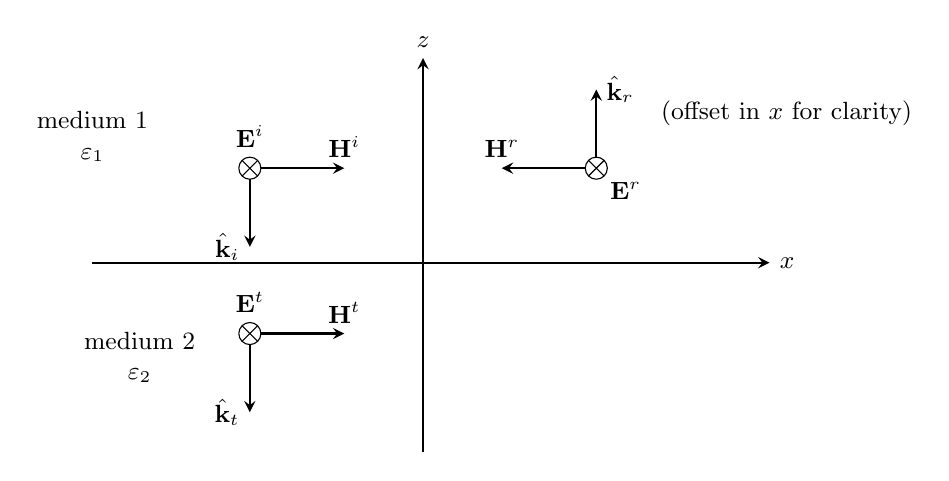
\begin{tikzpicture}[>=stealth, font=\small]
		% axes
		\draw[->, thick] (-4.2,0) -- (4.4,0) node[right] {$x$};
		\draw[->, thick] (0,-2.4) -- (0,2.6) node[above] {$z$};
		% media labels
		\node[align=center] at (-4.2,1.6) {medium 1\\$\varepsilon_1$};
		\node[align=center] at (-3.6,-1.2) {medium 2\\$\varepsilon_2$};
		% incident wave
		\begin{scope}[shift={(-2.2,1.2)}]
			\draw (0,0) circle (0.14);
			\draw (-0.1,-0.1) -- (0.1,0.1) (-0.1,0.1) -- (0.1,-0.1);
			\node[above] at (0,0.14) {$\mathbf{E}^i$};
			\draw[->, thick] (0.14,0) -- (1.2,0) node[above] {$\mathbf{H}^i$};
			\draw[->, thick] (0,-0.14) -- (0,-1.0) node[left] {$\hat{\mathbf{k}}_i$};
		\end{scope}
		% reflected wave
		\begin{scope}[shift={(2.2,1.2)}]
			\draw (0,0) circle (0.14);
			\draw (-0.1,-0.1) -- (0.1,0.1) (-0.1,0.1) -- (0.1,-0.1);
			\node[below right] at (0.05,-0.05) {$\mathbf{E}^r$};
			\draw[->, thick] (-0.14,0) -- (-1.2,0) node[above] {$\mathbf{H}^r$};
			\draw[->, thick] (0,0.14) -- (0,1.0) node[right] {$\hat{\mathbf{k}}_r$};
		\end{scope}
		\node[anchor=west] at (2.9,1.9) {(offset in $x$ for clarity)};
		% transmitted wave
		\begin{scope}[shift={(-2.2,-0.9)}]
			\draw (0,0) circle (0.14);
			\draw (-0.1,-0.1) -- (0.1,0.1) (-0.1,0.1) -- (0.1,-0.1);
			\node[above] at (0,0.14) {$\mathbf{E}^t$};
			\draw[->, thick] (0.14,0) -- (1.2,0) node[above] {$\mathbf{H}^t$};
			\draw[->, thick] (0,-0.14) -- (0,-1.0) node[left] {$\hat{\mathbf{k}}_t$};
		\end{scope}
	\end{tikzpicture}
	\caption{A uniform plane wave normally incident on the planar interface ($z = 0$) between medium 1 and medium 2. The $\mathbf{E}$ fields point along $+\hat{\mathbf{y}}$ (into the page). The incident, reflected, and transmitted waves are offset in $x$ for clarity.}
	\label{f:normal}
\end{figure}

We define the fields (phasors) as
\begin{align}
	\text{medium 1, incident:} \quad &
	\tilde{\mathbf{E}}^i = \hat{\mathbf{y}}E^i\,e^{\gamma_1 z}, &
	\tilde{\mathbf{H}}^i &= \hat{\mathbf{x}}\frac{E^i}{\eta_1}\,e^{\gamma_1 z}, \label{e:fields_i}\\
	\text{medium 1, reflected:} \quad &
	\tilde{\mathbf{E}}^r = \hat{\mathbf{y}}E^r\,e^{-\gamma_1 z}, &
	\tilde{\mathbf{H}}^r &= -\hat{\mathbf{x}}\frac{E^r}{\eta_1}\,e^{-\gamma_1 z}, \label{e:fields_r}\\
	\text{medium 2, transmitted:} \quad &
	\tilde{\mathbf{E}}^t = \hat{\mathbf{y}}E^t\,e^{\gamma_2 z}, &
	\tilde{\mathbf{H}}^t &= \hat{\mathbf{x}}\frac{E^t}{\eta_2}\,e^{\gamma_2 z}, \label{e:fields_t}
\end{align}
where (Lecture 2)
\begin{equation}
	\gamma_1 = \alpha_1 + j\beta_1, \quad \eta_1 = \frac{\eta_0}{\sqrt{\varepsilon_1}},
	\qquad\qquad
	\gamma_2 = \alpha_2 + j\beta_2, \quad \eta_2 = \frac{\eta_0}{\sqrt{\varepsilon_2}}.
\end{equation}
The total fields in each medium are
\begin{equation}
	\tilde{\mathbf{E}}_1 = \tilde{\mathbf{E}}^i + \tilde{\mathbf{E}}^r, \qquad
	\tilde{\mathbf{H}}_1 = \tilde{\mathbf{H}}^i + \tilde{\mathbf{H}}^r, \qquad
	\tilde{\mathbf{E}}_2 = \tilde{\mathbf{E}}^t, \qquad
	\tilde{\mathbf{H}}_2 = \tilde{\mathbf{H}}^t.
\end{equation}

\subsection{Boundary conditions and the Fresnel coefficients}

\begin{itemize}
	\item At $z = 0$, we must apply the BCs from Maxwell's equations.
	% NOTE: "always transverse" qualified to plane waves, as above.
	\item At normal incidence, the fields are entirely tangential to the interface (again, because EM plane waves are always transverse), so
	\begin{align}
		E^i + E^r &= E^t \qquad \rightarrow \text{tangential component of the $\mathbf{E}$ field conserved},\\
		\frac{E^i}{\eta_1} - \frac{E^r}{\eta_1} &= \frac{E^t}{\eta_2} \qquad \rightarrow \text{tangential component of the $\mathbf{H}$ field conserved}.
	\end{align}
	\item In general in RS, we know $E^i$, so we solve for the reflection and transmission coefficients
	\begin{equation}
		\rho = \frac{E^r}{E^i} \qquad \text{and} \qquad \tau = \frac{E^t}{E^i}.
	\end{equation}
	\item From above, we see
	\begin{equation}
		1 + \rho = \tau \qquad \text{and} \qquad 1 - \rho = \frac{\eta_1}{\eta_2}\tau.
	\end{equation}
	\item Solving gives the \emph{Fresnel reflection ($\rho$) and transmission ($\tau$) coefficients for normal incidence}:
	\begin{equation}
		\label{e:fresnel}
		\rho = \frac{\eta_2 - \eta_1}{\eta_2 + \eta_1} = \frac{\sqrt{\varepsilon_1} - \sqrt{\varepsilon_2}}{\sqrt{\varepsilon_1} + \sqrt{\varepsilon_2}},
		\qquad
		\tau = \frac{2\eta_2}{\eta_2 + \eta_1} = \frac{2\sqrt{\varepsilon_1}}{\sqrt{\varepsilon_1} + \sqrt{\varepsilon_2}}
	\end{equation}
\end{itemize}

\subsection{Connecting to the string model}

You may notice the similarity of forms between $\rho$ and $\tau$ and reflection and transmission on strings. Connecting to the string model given at the beginning of the lecture, consider \emph{lossless} media ($\varepsilon_1 = \varepsilon_1'$ and $\varepsilon_2 = \varepsilon_2'$) and recall that
\begin{equation}
	u_{p1} = \frac{c}{\sqrt{\varepsilon_1}} \qquad \text{and} \qquad u_{p2} = \frac{c}{\sqrt{\varepsilon_2}},
\end{equation}
so
\begin{equation}
	\rho = \frac{u_{p2} - u_{p1}}{u_{p2} + u_{p1}} = \frac{k_1 - k_2}{k_1 + k_2},
	\qquad
	\tau = \frac{2u_{p2}}{u_{p2} + u_{p1}} = \frac{2k_1}{k_1 + k_2},
\end{equation}
which are identical to the reflection and transmission coefficients on a string!

\subsubsection{$\star$ Key take-away point}

% NOTE: handwritten states the in-phase/out-of-phase rule "for general media"; it is exact for lossless media (rho real).
% For lossy media rho is complex and the phase is only near 0 or pi: e.g., for eps_1 = 1 and eps_2 = 70 - j30,
% rho = -0.797 + j0.037, a phase of 177 deg (python3 check of Eq. e:fresnel). It can depart substantially when losses
% are large relative to the contrast in n': eps_1 = 1, eps_2 = 3 - j3 gives 154 deg; eps_1 = 4, eps_2 = 4 - j4 gives
% 114 deg (python3). Worse, the Re(sqrt(eps)) criterion can pick the wrong branch for lossy media: eps_1 = 9,
% eps_2 = 4 - j12 gives Re sqrt(eps_1) = 3.00 > Re sqrt(eps_2) = 2.89 but arg rho = 106 deg. Exact general result (derived):
% rho = (a - b)/(a + b) with a = sqrt(eps_1), b = sqrt(eps_2) gives Re(rho) = (|eps_1| - |eps_2|)/|a + b|^2.
% Scoped the rule to lossless media and stated the exact criterion for lossy media.
The reflected EM wave is
\begin{itemize}
	\item in phase with the incident wave if
	\begin{equation}
		u_{p1} < u_{p2} \quad\Rightarrow\quad \mathrm{Re}\left(\sqrt{\varepsilon_1}\right) > \mathrm{Re}\left(\sqrt{\varepsilon_2}\right);
	\end{equation}
	\item out of phase ($\pi$ offset) with the incident wave if
	\begin{equation}
		u_{p1} > u_{p2} \quad\Rightarrow\quad \mathrm{Re}\left(\sqrt{\varepsilon_1}\right) < \mathrm{Re}\left(\sqrt{\varepsilon_2}\right),
	\end{equation}
	which is virtually always the case when medium 1 is the atmosphere.
	\item These conditions are exact for lossless media, where $\rho$ is real and the phase offset is exactly 0 or $\pi$. For lossy media, $\rho$ is complex and the offset lies in between. In general, $\mathrm{Re}(\rho) = (|\varepsilon_1| - |\varepsilon_2|)/|\sqrt{\varepsilon_1} + \sqrt{\varepsilon_2}|^2$, so the reflected wave is closer to in phase ($\mathrm{Re}(\rho) > 0$) when $|\varepsilon_1| > |\varepsilon_2|$ and closer to out of phase ($\mathrm{Re}(\rho) < 0$) when $|\varepsilon_1| < |\varepsilon_2|$. For air over water, ice, or soil, $|\varepsilon_2| \gg |\varepsilon_1|$, so the offset is near $\pi$.
\end{itemize}

\subsection{Power: reflectivity and transmissivity}

% NOTE: added "Using the time-averaged Poynting vector (Lecture 2) and writing E^r = y rho E_0^i e^{-gamma_1 z}" and, below,
% "the sum of the incident and reflected power densities" as minimal clarifications (cf. Ulaby & Long 2014, Eqs. 2.91, 2.92a).
We may also want to think about this in terms of the partitioning of energy between the reflected and transmitted waves. Using the time-averaged Poynting vector (Lecture 2) and writing $\tilde{\mathbf{E}}^r = \hat{\mathbf{y}}\rho E^i e^{-\gamma_1 z}$, we have in medium 1
% NOTE: added the assumption that medium 1 is lossless (gamma_1 = j beta_1, eta_1 real), as in Ulaby & Long (2014,
% Sec. 2-6.1, Eq. 2.91). The handwritten conjugate H_1^* = x (E_0^{i*}/eta_1)(e^{-gamma_1 z} - rho^* e^{gamma_1 z}) is
% correct only in that case (in general it is (E_0^{i*}/eta_1^*)(e^{gamma_1^* z} - rho^* e^{-gamma_1^* z})). For a lossy
% medium 1, the z = 0 result below gains a cross term: -2 Im(rho) sin(phi_eta1) is added to (1 - |rho|^2) cos(phi_eta1),
% and R + T != 1
% (e.g., eps_1 = 2 - j0.5, eps_2 = 20 - j10 gives R + T = 0.990; python3 check). The handwritten cos(phi_eta1) factors
% are kept; they equal 1 for a lossless medium 1. Medium 2 may be lossy.
\begin{align}
	\boldsymbol{\mathcal{S}}_{\mathrm{av}1} &= \frac{1}{2}\mathrm{Re}\left[\tilde{\mathbf{E}}_1\times\tilde{\mathbf{H}}_1^*\right] \nonumber\\
	&= \frac{1}{2}\mathrm{Re}\left[\hat{\mathbf{y}}E^i\left(e^{\gamma_1 z} + \rho\,e^{-\gamma_1 z}\right)\times\hat{\mathbf{x}}\frac{E^{i*}}{\eta_1}\left(e^{-\gamma_1 z} - \rho^*e^{\gamma_1 z}\right)\right],
\end{align}
taking medium 1 to be lossless ($\gamma_1 = j\beta_1$, $\eta_1$ real; e.g., the atmosphere), while medium 2 may be lossy. At $z = 0$, this gives
\begin{equation}
	\boldsymbol{\mathcal{S}}_{\mathrm{av}1} = -\hat{\mathbf{z}}\,\frac{|E^i|^2}{2|\eta_1|}\underbrace{\left(1 - |\rho|^2\right)}_{\text{note this term!}}\cos\phi_{\eta_1}
	= \boldsymbol{\mathcal{S}}^i_\mathrm{av} + \boldsymbol{\mathcal{S}}^r_\mathrm{av},
\end{equation}
the sum of the incident and reflected power densities. Similarly,
\begin{equation}
	\boldsymbol{\mathcal{S}}^t_\mathrm{av} = \boldsymbol{\mathcal{S}}_{\mathrm{av}2} = \frac{1}{2}\mathrm{Re}\left[\tilde{\mathbf{E}}_2\times\tilde{\mathbf{H}}_2^*\right]
	= -\hat{\mathbf{z}}\,|\tau|^2\frac{|E^i|^2}{2|\eta_2|}\cos\phi_{\eta_2}
\end{equation}
at $z = 0$, where $\phi_{\eta_1}$ and $\phi_{\eta_2}$ are the phase angles of $\eta_1$ and $\eta_2$ (Lecture 2). From these expressions, we can show
\begin{equation}
	|\tau|^2 = \frac{|\eta_2|\cos\phi_{\eta_1}}{|\eta_1|\cos\phi_{\eta_2}}\left(1 - |\rho|^2\right)
\end{equation}
and
\begin{equation}
	\boldsymbol{\mathcal{S}}_{\mathrm{av}1} = \boldsymbol{\mathcal{S}}_{\mathrm{av}2} \qquad \text{(sanity check: energy is conserved!)}.
\end{equation}
Finally, it is common to define the reflectivity $\Gamma$ and transmissivity $\mathbb{T}$,
% NOTE: handwritten writes R = S_0^r / S_0^i and T = S_0^t / S_0^i; written as the magnitudes of the time-averaged
% power densities at z = 0.
\begin{equation}
	\label{e:RT}
	\Gamma = \frac{\left|\boldsymbol{\mathcal{S}}^r_\mathrm{av}\right|}{\left|\boldsymbol{\mathcal{S}}^i_\mathrm{av}\right|}\bigg|_{z=0} = |\rho|^2
	\qquad \text{and} \qquad
	\mathbb{T} = \frac{\left|\boldsymbol{\mathcal{S}}^t_\mathrm{av}\right|}{\left|\boldsymbol{\mathcal{S}}^i_\mathrm{av}\right|}\bigg|_{z=0} = |\tau|^2\frac{|\eta_1|\cos\phi_{\eta_2}}{|\eta_2|\cos\phi_{\eta_1}},
\end{equation}
where it can be shown that
\begin{equation}
	\Gamma + \mathbb{T} = 1.
\end{equation}

%%%%%%%%%%%%%%%%%%%%%%%%%%%%%%%%%%%%%
% Symbols follow the master table in ../variables_master.tex; see it for flagged dual usages.
\section*{Variables}

Units are SI. Values are given for universal constants; ``typical'' values are representative, not definitive.

{\small
\renewcommand{\arraystretch}{1.25}
\begin{longtable}{>{$}l<{$} >{\raggedright\arraybackslash}p{0.37\textwidth} >{\raggedright\arraybackslash}p{0.15\textwidth} >{\raggedright\arraybackslash}p{0.24\textwidth}}
\hline
\textrm{Symbol} & Description & Units & Value \\
\hline
\endfirsthead
\hline
\textrm{Symbol} & Description & Units & Value \\
\hline
\endhead
\hline
\endfoot
\multicolumn{4}{l}{\emph{Universal constants}} \\
\varepsilon_0 & permittivity of free space & F/m & $8.854\times10^{-12}$ \\
\mu_0 & permeability of free space & H/m & $4\pi\times10^{-7} \approx 1.257\times10^{-6}$ \\
c & speed of light in a vacuum, $1/\sqrt{\mu_0\varepsilon_0}$ & m/s & $2.998\times10^{8}$ \\
\eta_0 & intrinsic impedance of free space, $\sqrt{\mu_0/\varepsilon_0}$ & $\Omega$ & $\approx 376.7$ ($\approx 120\pi$) \\
j & imaginary unit, $j^2 = -1$ (time dependence $e^{j\omega t}$) & -- & -- \\
\multicolumn{4}{l}{\emph{Constitutive parameters}} \\
\varepsilon & complex dielectric constant (relative), $\varepsilon' - j\varepsilon''$ & dimensionless & -- \\
\varepsilon' & relative permittivity (real part of $\varepsilon$) & dimensionless & $\ge 1$ (almost always) \\
\varepsilon_1,\ \varepsilon_2 & dielectric constants of media 1 and 2 & dimensionless & -- \\
\mu & magnetic permeability & H/m & $\approx\mu_0$ in RS \\
\mu_1,\ \mu_2 & permeabilities of media 1 and 2 & H/m & $\mu_0$ in RS \\
\sigma_1,\ \sigma_2 & conductivities of media 1 and 2 & S/m & -- \\
\omega & angular frequency (set by the source) & rad/s & -- \\
\multicolumn{4}{l}{\emph{Waves on strings}} \\
\xi & transverse displacement of the string & m & -- \\
\xi^i,\ \xi^r,\ \xi^t & incident, reflected, and transmitted waves on the strings & m & -- \\
\xi_0^i,\ \xi_0^r,\ \xi_0^t & complex amplitudes of $\xi^i$, $\xi^r$, $\xi^t$ & m & -- \\
\phi^i,\ \phi^r,\ \phi^t & phases of $\xi_0^i$, $\xi_0^r$, $\xi_0^t$ & rad & $\phi^t = \phi^i$ \\
F_\mathrm{tension} & string tension ($F_{\mathrm{tension},1}$, $F_{\mathrm{tension},2}$ for strings 1 and 2) & N & equal in both strings \\
m_\ell,\ m_{\ell 1},\ m_{\ell 2} & mass per unit length of the string (of strings 1 and 2) & kg/m & -- \\
u_p & phase velocity; on a string, $\sqrt{F_\mathrm{tension}/m_\ell}$; EM waves, $c/n'$ & m/s & -- \\
u_{p1},\ u_{p2} & phase velocities in strings (media) 1 and 2 & m/s & lossless EM: $c/\sqrt{\varepsilon_{1,2}}$ \\
k_1,\ k_2 & angular wavenumbers in strings (media) 1 and 2, $\omega/u_p$ & rad/m & -- \\
z & coordinate along the string; normal to the interface (EM) & m & interface at $z = 0$ \\
t & time & s & -- \\
n' & real part of the index of refraction, $\mathrm{Re}(\sqrt{\varepsilon})$ & dimensionless & -- \\
\multicolumn{4}{l}{\emph{Boundary conditions}} \\
\mathbf{E},\ \mathbf{H} & electric and magnetic field intensity vectors (instantaneous) & V/m; A/m & -- \\
\mathbf{E}_1,\ \mathbf{E}_2 & (total) electric field in media 1 and 2 & V/m & -- \\
\mathbf{H}_1,\ \mathbf{H}_2 & (total) magnetic field in media 1 and 2 & A/m & -- \\
E^\perp,\ H^\perp & field components perpendicular (normal) to the interface & V/m; A/m & -- \\
E^\parallel,\ H^\parallel & field components parallel (tangential) to the interface & V/m; A/m & -- \\
\mathcal{V},\ \partial\mathcal{V} & volume and its closed bounding surface (Gauss's laws) & m$^3$; m$^2$ & -- \\
\mathcal{A},\ \partial\mathcal{A} & open surface of integration and the closed loop bounding it & m$^2$; -- & -- \\
d\mathbf{a} & vector area element & m$^2$ & -- \\
\hat{\mathbf{a}} & unit normal to the interface, from medium 2 to medium 1 & dimensionless & -- \\
d\boldsymbol{\ell} & vector line element along $\partial\mathcal{A}$ & m & -- \\
\ell,\ \boldsymbol{\ell} & length (and vector) of the long side of the loop & m & -- \\
I_f & free current through the loop & A & 0 (assumed) \\
\multicolumn{4}{l}{\emph{Normal incidence}} \\
\tilde{\mathbf{E}}^i,\ \tilde{\mathbf{E}}^r,\ \tilde{\mathbf{E}}^t & phasors of the incident, reflected, and transmitted electric fields & V/m & -- \\
\tilde{\mathbf{H}}^i,\ \tilde{\mathbf{H}}^r,\ \tilde{\mathbf{H}}^t & phasors of the incident, reflected, and transmitted magnetic fields & A/m & -- \\
\tilde{\mathbf{E}}_1,\ \tilde{\mathbf{H}}_1 & total field phasors in medium 1 & V/m; A/m & -- \\
\tilde{\mathbf{E}}_2,\ \tilde{\mathbf{H}}_2 & total field phasors in medium 2 & V/m; A/m & -- \\
E^i,\ E^r,\ E^t & complex amplitudes of the incident, reflected, and transmitted $\mathbf{E}$ fields at $z = 0$ & V/m & $E^i$ known \\
\hat{\mathbf{k}}_i,\ \hat{\mathbf{k}}_r,\ \hat{\mathbf{k}}_t & propagation unit vectors of the incident, reflected, and transmitted waves & dimensionless & $-\hat{\mathbf{z}}$, $\hat{\mathbf{z}}$, $-\hat{\mathbf{z}}$ \\
\hat{\mathbf{x}},\ \hat{\mathbf{y}},\ \hat{\mathbf{z}} & Cartesian unit vectors & dimensionless & -- \\
\gamma_1,\ \gamma_2 & propagation constants of media 1 and 2, $\alpha + j\beta$ & m$^{-1}$ & -- \\
\alpha_1,\ \alpha_2 & attenuation constants of media 1 and 2 & Np/m & 0 if lossless \\
\beta_1,\ \beta_2 & phase constants of media 1 and 2 & rad/m & $k_{1,2}$ if lossless \\
\eta_1,\ \eta_2 & intrinsic impedances of media 1 and 2, $\eta_0/\sqrt{\varepsilon_{1,2}}$ & $\Omega$ & real if lossless \\
\phi_{\eta_1},\ \phi_{\eta_2} & phase angles of $\eta_1$ and $\eta_2$ & rad & 0 if lossless \\
\rho & Fresnel reflection coefficient (normal incidence), $E^r/E^i$ & dimensionless & $|\rho| \le 1$ \\
\tau & Fresnel transmission coefficient (normal incidence), $E^t/E^i$ & dimensionless & $1 + \rho$ \\
\boldsymbol{\mathcal{S}}_{\mathrm{av}1},\ \boldsymbol{\mathcal{S}}_{\mathrm{av}2} & time-averaged power density (Poynting vector) in media 1 and 2 & W/m$^2$ & equal at $z = 0$ \\
\boldsymbol{\mathcal{S}}^i_\mathrm{av},\ \boldsymbol{\mathcal{S}}^r_\mathrm{av},\ \boldsymbol{\mathcal{S}}^t_\mathrm{av} & time-averaged power densities of the incident, reflected, and transmitted waves & W/m$^2$ & -- \\
\Gamma & reflectivity, $|\rho|^2$ & dimensionless & $0 \le \Gamma \le 1$ \\
\mathbb{T} & transmissivity, $1 - \Gamma$ (medium 1 lossless) & dimensionless & $0 \le \mathbb{T} \le 1$ \\
\end{longtable}
}

\end{document}
